\section{Convergence of the Method}
\label{sec:convergence}

The above halo-based metrics will have a certain level of dependence on the
choice of halo finder used. In an attempt to ensure independence of the results
from such factors, the above analysis was repeated both with the 3D
friends-of-friends halo finder included in the {\tt yt} package \citep{Turk2011}.
This is simpler than the \velociraptor{} method used for the main analysis, and
is unable to disentangle mergers. However, as active mergers make up a small
fraction of the galaxy population, the above results are qualitatively
unaffected and are only change quantitatively to the 5\% level. The above
analyses were also re-ran with the \velociraptor{} catalogue by re-finding
halos manually by selecting all particles within $R_{\rm BN98}$, the halo
radius as defined by \citet{Bryan1998}, of the halo center, rather than using
the non-spherical particles catalogue provided. This, again, left the results
qualitatively and quantitatively unchanged.


\subsection{Filling in Holes}


One valid criticism of our methodology for producing lagrangian regions is that
they are relatively spotty; simply using the dark matter particles from a given
halo naturally leads to a very diffuse lagrangian region. To remedy this, it is
possible to smooth out the lagrangian regions, by extending the procedure
that was used to extend the regions from the dark matter to the gas.
This works as follows:
\begin{enumerate}
	\item For every dark matter particle that does not end up in a halo 
	      in the initial conditions, find the nearest $n$ neighbours.
	\item Find among the neighbours the maximal lagrangian region ID,
	      corresponding to the lowest mass $z=0$ halo.
	\item Assign the particle the same lagrangian region ID.
\end{enumerate}
The choice to assign the particles to the lowest mass halo, rather than the
higher mass halo, was made to ensure that spurious transfer into the lower mass
halo was avoided wherever possible. This means that the expectation is that
with this metric the level of inter-lagrangian transfer will increase with
respect to the fiducial lagrangian region identification method. The results
with the particles given to the halos of a higher mass show negligible
deviation from the fiducial result.

\begin{figure}
	\centering
	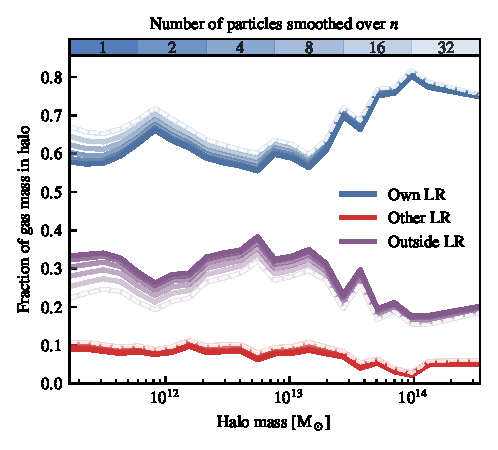
\includegraphics{figures/convergence_smoothing.pdf}
	\vspace{-0.7cm}
	\caption{The gas transfer mass function reproduced from Fig.
		\ref{fig:maintransferresult}. Each line, coded by transparency,
		shows the fraction of baryonic mass in a halo from each component
		when the lagrangian regions have been smoothed by 1 (i.e. the fiducial result), 2, 4, 8, 16,
		or 32 particles (from lightest to darkest respectively). The dashed
		line shows the result for the 32-smoothing case where the particles are
		given to the highest, rather than lowest, mass halos. See the
		text for the details of how this smoothing is constructed.
	}
	\label{fig:smoothconv}
\end{figure}

The results are shown in Fig. \ref{fig:smoothconv}. Note how smoothing the
lagrangian regions does have the expected effect of inducing more internal
transfer, and does increase the proportion of baryons that are classified
as retained as the lagrangian regions are filled out.

\subsection{The sizes of halos}

\blue{Currently there is a bug in the code that needs to be rectified before
this plot can be re-made with the current version of the code.}

\begin{figure}
    \centering
    \vspace{-0.5cm}
    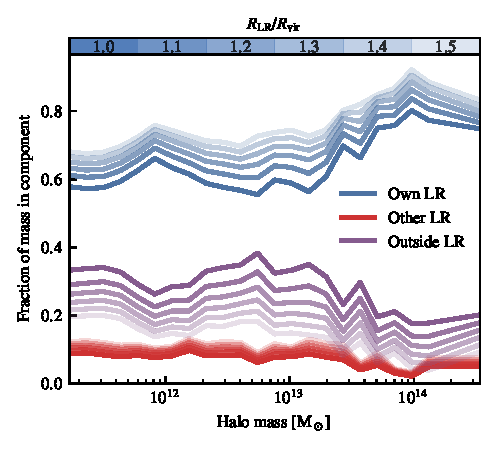
\includegraphics{report/figures/radius_convergence.pdf}
    \vspace{-0.5cm}
    \caption{Convergenece with increasing virial radius for the lagrangian region.
    \blue{TODO: note that these were made with AHF.} Darker colours correspond
    to large radii, going in steps of $0.1R_{\rm vir}$ from 1.0 to 1.5.}
    \label{fig:my_label}
\end{figure}

\begin{itemize}
	\item Virial radius dependence
		\begin{itemize}
			\item Transfer from outside dominated by nearby particles
			\item Must re-find halos to do this analysis
			\item Describe algorithm
			\item We have the plots!
			\item Not the case
		\end{itemize}
\end{itemize}
